% This is a sample document using the University of Minnesota, Morris, Computer Science
% Senior Seminar modification of the ACM sig-alternate style. Much of this content is taken
% directly from the ACM sample document illustrating the use of the sig-alternate class. Certain
% parts that we never use have been removed to simplify the example, and a few additional
% components have been added.

% See https://github.com/UMM-CSci/Senior_seminar_templates for more info and to make
% suggestions and corrections.

\documentclass{sig-alternate}
\usepackage{color}
\usepackage[colorinlistoftodos]{todonotes}

%%%%% Uncomment the following line and comment out the previous one
%%%%% to remove all comments
%%%%% NOTE: comments still occupy a line even if invisible;
%%%%% Don't write them as a separate paragraph
%\newcommand{\mycomment}[1]{}

\begin{document}

% --- Author Metadata here ---
%%% REMEMBER TO CHANGE THE SEMESTER AND YEAR AS NEEDED
\conferenceinfo{UMM CSci Senior Seminar Conference, December 2015}{Morris, MN}

\title{An Examination of Concurrent Compaction Techniques in JVM Garbage Collection}

\numberofauthors{1}

\author{
% The command \alignauthor (no curly braces needed) should
% precede each author name, affiliation/snail-mail address and
% e-mail address. Additionally, tag each line of
% affiliation/address with \affaddr, and tag the
% e-mail address with \email.
\alignauthor
Jacob P. Opdahl\\
	\affaddr{Division of Science and Mathematics}\\
	\affaddr{University of Minnesota, Morris}\\
	\affaddr{Morris, Minnesota, USA 56267}\\
	\email{opdah023@morris.umn.edu}
}

\maketitle
\begin{abstract}
This paper provides an overview of garbage collection (GC) of memory 
in programming languages and parallel processing as well as how 
parallel processing applies to GC; particularly, these
concepts are focused within the context of the Java Virtual Machine (JVM).
We examine in detail various algorithms that perform compaction of fragmented 
memory during garbage collection concurrently to the application running.
The desire for such GC behavior stems from a desire to reduce stop-the-world
pauses of an application.
% The current paper format *only* allows inline comments using the todo
% macro. That's kind of a bummer, and it would be neat if someone figured
% out how to change the acmconf style to allow this. I suspect it isn't *hard*
% but there are quite a few details that have to be sorted out in synchrony.
\end{abstract}

\keywords{Garbage Collection (GC), Concurrency, Compaction, Continuously Concurrent Compacting Collector (C4), Collie, Field Pinning Protocol (FPP)}

\section{Introduction}
\label{sec:introduction}

In object-oriented programming languages, the allocation and deallocation
of memory for objects can be explicit or implicit. If done implicitly,
a language is said to have \emph{automatic memory management}. Some languages 
with automatic memory management are C\#, Java, and Python.
Use of automatic memory management is beneficial to programmers as it provides
the robustness of an object-oriented language without worrying about
details unrelated to what their program is intended to do; specifically, they do
not have to worry about the details of memory allocation and deallocation. 
However, programmers also do not have control over how memory management occurs
, which can have negative impacts on application performance.

Memory for a program is not an unlimited resource. As such, automatic memory management
must ensure objects that are no longer needed are removed from memory
when appropriate. Dead objects, or \emph{garbage}, are objects that can be shown
to be unreachable by the program~\cite{glossary:g}. Thus, garbage should be deallocated to 
save space for new objects that will be created. The algorithm used to perform implicit
deallocation of garbage is referred to as a \emph{garbage collector}.
A garbage collector is a sophisticated algorithm designed to detect
and remove dead objects. We will focus on specific parts of the 
garbage collection (GC) process performed by different Java Virtual Machines 
(JVMs), software processes that run Java programs on computing systems~\cite{Lindblom:2011}.

\todo[inline]{Still need to talk briefly about why parallel GC is becoming necessary.
Might also want to say what kind of BG will be introduced and what algorithms I will look at? 
If I do, I will likely leave out implementation details of GC algorithms until their introductory
parts of their sections.}

\section{Background}
\label{sec:background}

\todo[inline]{Just threw stuff from outline in this section for now.}

This is where I explain terminology and aspects of GC and parallel 
computing that are necessary to understand my paper (If there is 
enough information in each subsection, I should maybe forego the 
background and just make them all sections)

\subsection{Garbage Collection}
\label{sec:garbageCollection}

References and the heap (if not done in the introduction)

General process flow GC algorithms tend to follow

Specific GC algorithms/techniques my researched papers will 
refer to and common techniques needed to understand my paper 
(Pauseless, tracing/marking, more)

Start introducing some terminology relevant to single processor 
garbage collectors such as: stop-the-world, fragmentation, compaction, 
tracing, reference remapping, etc.

Explain the three typical aspects of compaction 
(relocation/copying, remapping, and reclamation: 
reclamation is often just done through the other two)

\subsection{Parallel Processing}
\label{sec:parallelProcessing}

Threads: the virtual form of a processor (might need to 
explain virtualization or abstraction)

Issues experienced in parallel computing and reasons why it 
is difficult to perform effectively like: deadlock, race conditions, 
etc. (Real brief, but I feel the audience needs to have some idea of 
why progress in this area doesn't happen overnight. It also seems 
necessary for explaining barriers)

Typical ways of mitigating challenges experienced in parallel 
computing (synchronization, barriers/locks)

\todo[inline]{Decided a portion I wrote for Collie
should be included in the general background. Throwing what I wrote here
for now. Will be rewritten later.}
A \emph{global safepoint} is requested by a thread and is a moment when all 
threads are paused such that operations can be performed by the requesting thread without having to worry 
about references in the application changing. As a global safepoint requires pausing application
threads, this breaks concurrency.
Note that a safepoint differs from a barrier in GC. In a safepoint,
all threads are allowed to reach a certain point then their execution is simply paused.
A barrier works by telling threads how to behave if multiple try to access the same
memory. Thus, using a global safepoint does not break the goal of barrier-free compaction
~\cite{Humble:2015}.

Also, talk about checkpoints here.

\subsection{Parallel Processing as it Applies to Garbage Collection}
\label{sec:parallelProcessingGarbageCollection}

Bring audience's attention back to the original focus introduced 
of wanting to use parallel computing to improve GC

Introduce new terminology for GC that depends on parallel processing 
in order to show some more specific ways in which parallel processing 
can be used to improve GC (mutator threads, parallelism, concurrency, etc.)

Explain Latency vs throughput

Describe the focus: Concurrent Compaction (If this has enough information, 
it could be moved out of being a component in a subsection)


\section{The C4 Collector}
\label{sec:c4}

%I think I got enough introductory info describing the context of C4
%here. Might want to check with Elena.
The first concurrent compaction algorithm we examine is implemented in the 
Continuously Concurrent Compacting Collector (C4), which is a garbage collector 
included in JVMs commercially shipped by Azul Systems~\cite{Tene:C4}. The 
researchers, Iyengar et al., describe how C4 is an enhanced, generational variant
of the Pauseless garbage collector~\cite{Click:Pauseless}. C4 is generational in 
that the entire GC algorithm is independently utilized in both the young and old generations 
concurrently; in addition, both generations have garbage collected concurrently 
to the application running. For set condemnation, C4 uses a tracing-style algorithm.
C4 is intended to be used in server environments with multiple GB heaps and 
multiple GB/sec allocation rates.


\subsection{Loaded Value Barrier}
\label{sec:c4LVB}

C4 uses a barrier referred to as the \emph{Loaded Value Barrier} (LVB) to 
maintain concurrency throughout the GC process~\cite{Tene:C4}. The LVB 
places invariants on each object reference value as it is loaded from memory.
One of the invariants relates to the tracing portion of the GC algorithm, so
it is not discussed here. The other invariant states that a loaded
reference value must point to the location of the object that currently has the
object's contents that are safely accessible. 
In other words, if an object is being relocated, references to it must point 
to the the object wherever it can be safely accessed, be it the from or to 
space. If the invariant does not hold
when a reference is loaded, the barrier will trigger and execute code to correct
the situation. The code executed depends on what causes the trigger
and is discussed later.

In order to prevent repetitive barrier triggers from a single incorrect reference,
the LVB uses a \emph{self-healing} technique. Whenever a reference triggers LVB
due to the reference not meeting an invariant, it will perform the rectifying code
necessary to fix the reference. Additionally, the barrier will go to the memory
location the reference was loaded from and fix the the source of the reference. This
ensures not only the loaded reference being used is fixed, but the stored reference
that might be loaded again later is also fixed. This is possible because the LVB 
is checked directly following reference load but before the reference is used.
Self-healing helps reduce the occurrence of the read barrier triggers.


\subsection{Concurrent Relocation}
\label{sec:c4Relocation}

The relocation aspect of compaction in the Collie occurs on a per-\emph{page}
basis, where a page is a fixed-length, contiguous block of virtual memory
that is backed by a contiguous block of physical storage~\cite{wiki:page}\cite{Tene:C4}.
To quickly empty virtual pages, the most sparsely populated pages are relocated
first. The from space in this relocation is actually from pages, and the to space
is to pages. From pages are pages with garbage
and are marked as such during the tracing phase.

% Maybe could get rid of this later if space is needed and just stick to the pseudocode.
To support concurrent relocation, pages being relocated are protected. 
The LVB will trigger for mutator threads encountering a reference pointing to an object
on a protected page. If the object has been relocated already, LVB will
obtain the new location for the mutator. If the object is being relocated, 
LVB will cause the mutator to wait
for the GC thread to finish before continuing to work.
If the object has not started relocation, LVB has the mutator thread 
escalate its movement status by moving the object itself. After any of 
these situations, the LVB will also cause the mutator thread to update 
the reference to the new location and heal the source location of the reference.
Without any mutator accesses, the GC threads will relocate the objects but
will not remap references at this time. If an object
spans multiple pages, \emph{page shattering} is used to relocate chunks of
it at a time sequentially while minimizing interruptions to mutators;
finer details of this can be read here~\cite{Tene:C4}.

When all living objects are relocated from a page marked for relocation,
the C4 compactor will utilize a \emph{Quick Release} method. In order to quickly recycle
physical memory sources, the physical memory backing the page will be marked as freed
as soon as the last object has been moved to a to page. Because the objects have already 
been transferred to new page, the contents of the from pages are no longer needed. Thus,
the physical memory backing it can be put to use immediately. The from page's virtual 
addresses will be in use until all references have been remapped, but this 
allows for efficient recycling of physical memory. This is made possible as the C4 compactor
stores object forwarding information outside of a from page. Thus, when a reference to
a from page is loaded, LVB has the mutator check the forwarding table rather than the
from page to see where an object has moved to.

The key point here is GC threads do the most work. They simply
move objects from the from pages. Meanwhile, the LVB protects pages being 
relocated with the previously mentioned invariant. The LVB is checked for every reference load
done by a mutator thread, so every time a thread adds a reference to its 
stack or register. In the case of compaction, we care if the mutator is trying 
to access an object on a protected page. If it is, the barrier will trigger 
handling code. This can be seen in the pseudocode. Assuming the issue with the
reference came from compaction, as opposed to tracing, the object the reference
points to will be checked for its relocation state; if it has not been relocated, the
thread will relocate it. Once the thread knows it has been relocated, by itself
or a GC thread, it will update get the object's relocated position. Using this,
a method is performed to change the original location
the invalid reference was loaded from (this is also performed for tracing triggers).

\todo[inline]{Get some nice way of showing pseudocode...}


\subsection{Concurrent Remapping}
\label{sec:c4Remapping}

To maintain concurrency while updating all references to the now relocated
objects, the C4 compaction algorithm uses two techniques~\cite{Tene:C4}. The first is
referred to as \emph{lazy remapping}. This essentially allows the mutator
threads to continue updating references as they trigger the LVB. In order for
the remapping phase of compacting GC to end, all live references must be updated.
This could go on indefinitely if lazy remapping alone is relied upon.

To finish remapping, a traversal of live references must be performed to
ensure they are all updated, like the traversal performed to trace which
objects are now garbage. Since no physical resources are being held due
to Quick Release and lazy remapping does not disrupt mutator operations,
the remapping traversal is pushed off until another GC cycle starts. That
is, C4 will have the remapping of one GC cycle be performed while the tracing
of another cycle is beginning. This works since both processes need to traverse
the same object and reference graphs to find all reachable references. To
visualize how this works, examine Figure~\ref{fig:c4Cycle}.

\todo[inline]{Make the figure greyscale/black-and-white accessible.}

\begin{figure}
\centering
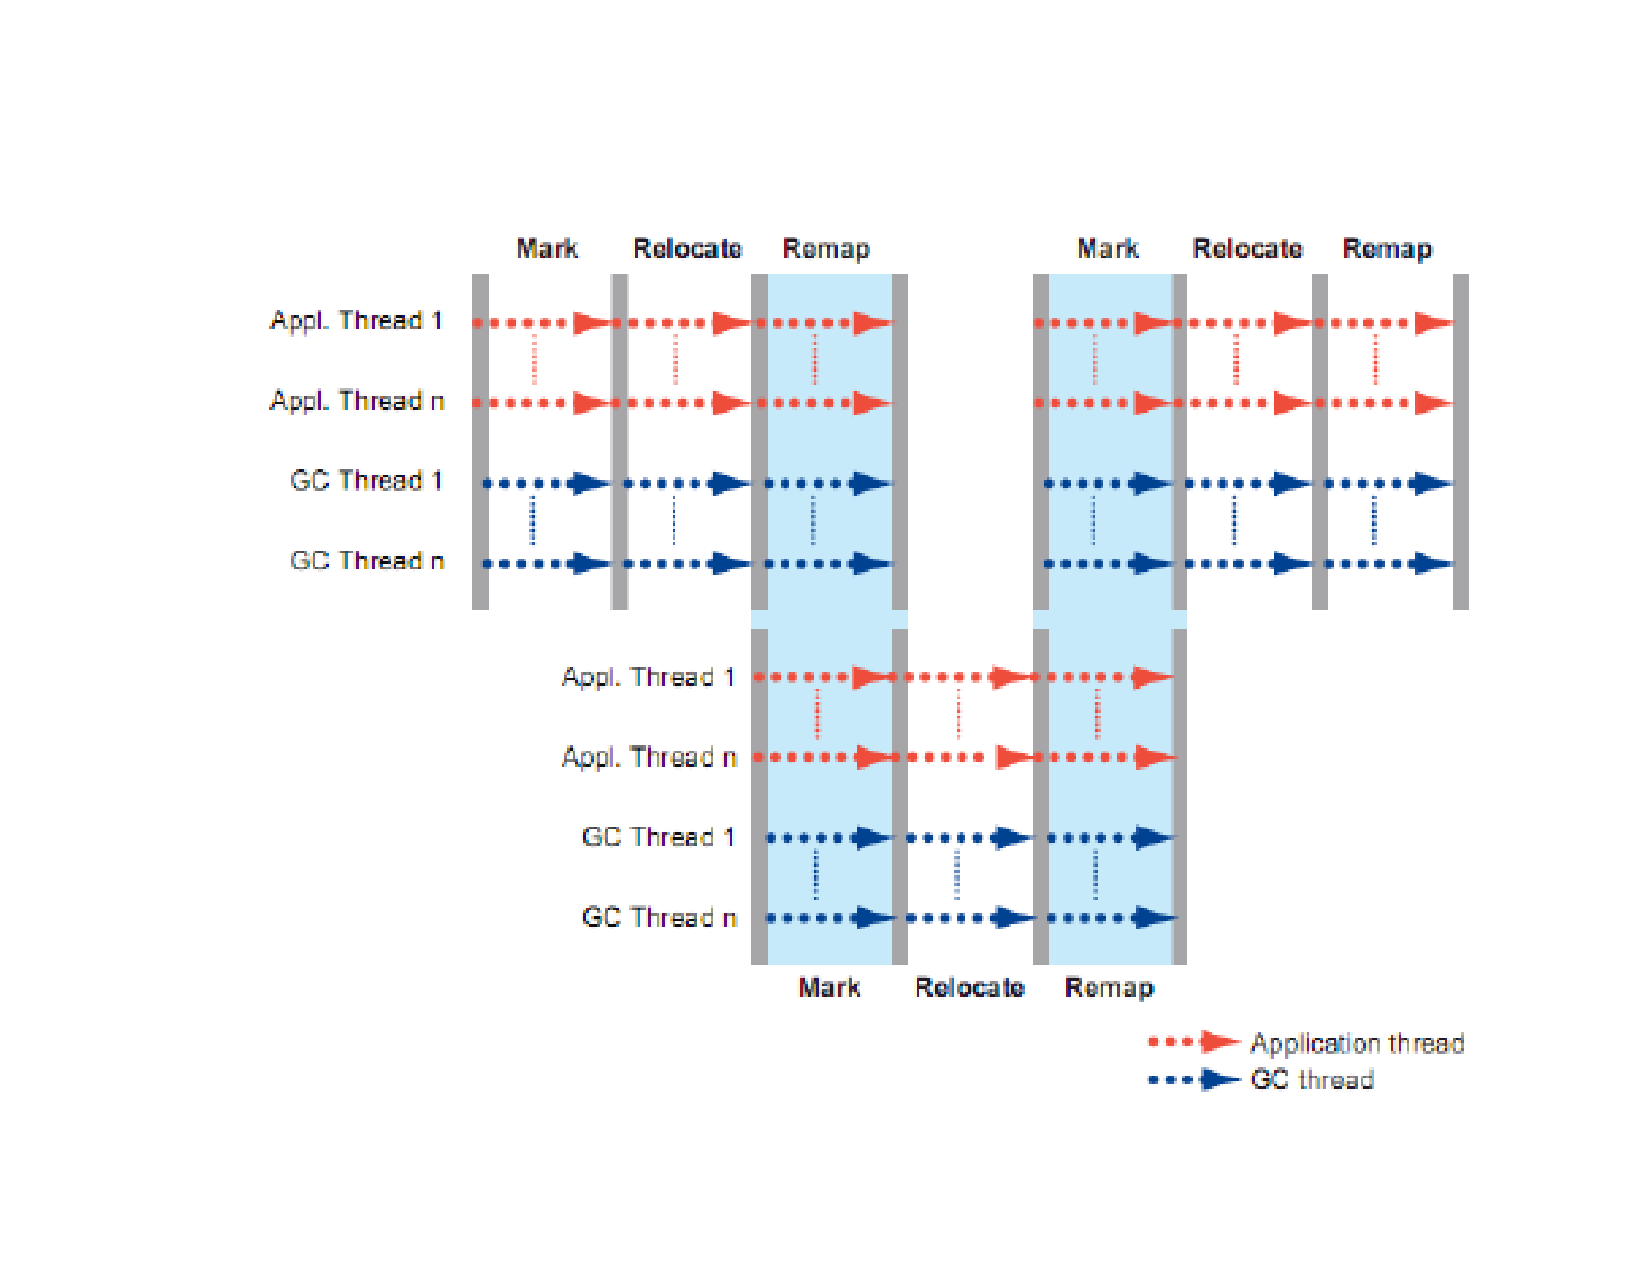
\psfig{file=c4Mapping_rough_figure.pdf,width =3in}
\caption{C4 GC cycle. Remapping and Tracing are rolled into one traversal.
(taken from \cite{Tene:C4})}
\label{fig:c4Cycle}
\end{figure}


\subsection{C4 Results Summary}
\label{sec:c4Results}

Experiments done with the implemented C4 algorithm were meant to show the
benefits of using an algorithm that is simultaneously generational and concurrent~\cite{Tene:C4}.
C4 is tested against a modified C4 algorithm that is not generational. Additionally,
it is tested against two algorithms that do not perform concurrent compaction. 
All GC algorithms were tested on the same hardware; the setup was a
2 socket, 12 core Intel x5680 server with 96 GB of memory. The test exhibited
an allocation rate of about 1.2GB/sec, and there were live sets of objects on 
the heap consistently at a size of around 2.5GB; the actual heap size was allowed 
to grow though, indicating greater amounts of garbage on the heap. The applications were run long
enough to ensure multiple full heap GC cycles were performed and at least one
significant compaction event occurred.

The primary performance metric monitored was the worst-case response times
of the servers responding to requests while experiencing the workloads
described above. This gives a sense of how much garbage collection slows
an application's responses to clients. C4 maintained the smallest 
range of worst-case response times and it did so across the largest range of heap sizes.
The worst-case response times were usually in the range of 0.01-0.1secs. 
These response times are fast enough to be considered \emph{pauseless}. 
The non-generational version of C4 could also reach pauseless thresholds,
but the range of heap sizes it could do so for was far more limited. Where standard
C4 sustained pauseless operation for heap sizes of 5-35GB, the modified C4 could
only do so for heaps sizes of 15-35GB. The non-concurrently compacting
collectors had multi-second worst-case response times for all heap sizes experienced.


\section{The Collie Collector}
\label{sec:collie}

\todo[inline]{Implemented some feedback received from Elena on the section draft. Mostly just removed
the subsubsection on the theoretical implementation. Still need to
update the introduction to explain who the creators are, that they are the same as those who made C4,
if the algorithm has actually been implemented and where, what the type of environment is it is defined for,
that it pulls a lot from C4, etc. Also, need to think of where figures and examples can be used. Need
to make sure there are no references (haha) to the old theoretical section I had. Need to make sure
all things that need background info receive it earlier (make a list). Need to update results with numbers
and remove the conclusion-y stuff for the conclusion section. Basically, if you're a professor or adviser 
and you read this for the section draft, it's not worth reading again yet.}
\todo[inline, color=green]{Stuff I've worked on modifying from the above list: introduction.}

\todo[inline]{Also, consider what aspects of Collie directly come from C4 as well as which ones are
important/different enough to talk about once again.}

We now look at the concurrent compaction technique used within the 
Collie garbage collector described by Iynegar et al.~\cite{Iyengar:Collie};
with the exception of Gehringer, they were the researchers who worked on the C4 algorithm.
As such, Collie utilizes modified versions of several techniques within C4, such as:
the tracing algorithm, the LVB, page-granularity compaction, self-healing, and quick-release behavior.
Only the LVB is modified in significant ways for the purposes of compaction in Collie,
so the rest of the techniques are not re-discussed here. Additionally, the Collie
collector is also designed with server environments in mind. Collie is implemented and tested in 
the same production quality Azul JVM that the Pauseless garbage collector is implemented in~\cite{Click:Pauseless}. However, it has not been made commercially available.


\subsection{Transactional Memory}
\label{sec:collieTM}

The Collie's compaction algorithm sets itself apart due to its use 
of a \emph{transactional memory} (TM) system as a concurrency control 
alternative to barriers~\cite{Iyengar:Collie}. TM systems allow
sections of code to function 
analogously to \emph{transactions} from database systems, 
which are a series of operations performed as one unit where 
they occur in an all-or-none manner~\cite{wiki:atomicity}.

For example, consider updating the inventory of a store; this may involve updating
the price, quantity and distributor for various items. 
If a person was updating information regarding an item, they would 
want all three attributes of the item to be updated or none at all. Having
only a subset of the attributes updated could cause confusion.

TM systems allow a series
of operations that modify memory to be placed in
a \emph{transactional procedure}, much like a database transaction.
The TM system then monitors the access of concurrent threads to \emph{transactional variables}:
memory modified by a transactional procedure.
Concurrent threads will operate in parallel until they try to modify
the same transactional variable. At this time, behavior can be specified as to how 
the conflict should resolve, but the general pattern would be for one transaction
to be aborted and the other allowed to continue.
When a transaction is completed, its changes are \emph{committed}; any changes 
made to memory by the transaction are finalized~\cite{wiki:transactional-memory}.


\subsection{Object Transplantation}
\label{sec:collieTransplantation}

% Two possible changes to come here. If C4 also does reclamation the "easy way"
% as described by FPP, then mentioning it in background and elsewhere can probably
% be simplified to a simple note of that being how it's handled by all the algorithms
% I discuss. Also, Might not need the refresher on relocation and remapping if talked
% about recently before.
With the use of a TM system for synchronizing concurrent compaction,
new terminology is introduced for understanding the Collie 
compactor~\cite{Iyengar:Collie}. As discussed, compaction of
memory requires relocation of objects and remapping of references to
the objects; the Collie does reclamation by labeling the from-space as freed.
An object \emph{transplantation} consists of both the relocation and 
remapping of an object. A transplantation has not been completed until
the object's contents have been moved and all required references have been
updated. All relocating collectors, and by extension all
compacting collectors, transplant objects. The Collie compactor 
performs individual object transplantations within transactional procedures. 

Each object in an application's memory has a \emph{referrer set}. This is the precise set 
of all references pointing to the object. It is crucial that an object's referrer set not
be modified or expanded during the object's transplantation. Doing so could result
in references to the object being created that the transactional procedure
was not aware of when starting, so they are not updated to point to 
the new object location when it is finishing. To avoid this, a referrer set can be
\emph{protected} by writing to each reference within it and preventing it from
being read temporarily.

There is also a notion of a \emph{stable} referrer set. An object has a stable referrer 
set if the object's referrer set meets the following criteria:
\begin{enumerate}
\item Once the overall GC process begins, no references to the object may be written to the heap
\item At the start of the object's transplantation, no threads contain references to the object in their stacks/registers
\item Once transplantation is underway, no new references may be added to the object's \emph{transplantation state} until it is complete
\end{enumerate}
This ensures the compactor is aware of all references to the object
and the references to the object go unchanged.

An object has a transplantation state consisting of the object's contents 
and the object's referrer set. This definition builds on the general requirements
for completing an object transplantation. These
requirements include: all copies of an object's contents should remain consistent
until transplantation is completed and after transplantation, there cannot be any
references pointing to the object's from-space location in its referrer set.

%Note to self: consider removing chunk where I mention the general requirements for completing an individual
%object transplantation.


\subsection{The Collie Protocol}
\label{sec:collieAlgorithm}


\subsubsection{Aborting Compactor}
\label{sec:collieAbortion}

The compactor implemented in the Collie GC algorithm uses barriers 
and transactions that will abort the transplantation process of an object if the
GC threads and mutator threads conflict to maintain concurrency~\cite{Iyengar:Collie}.
However, objects that have their transplantation aborted would then be stuck
in from-space, which would mean compaction is never performed. This is why
the additions of a \emph{mirrored-to-space} and \emph{zero-copy transplantation} are necessary.

Mirrored-to-space is a virtual address space that corresponds to and is the same
size as from-space. Mirrored-to-space memory pages are mapped to the same physical
memory as their corresponding from-space pages are. For barrier test and compaction 
termination purposes, mirrored-to-space is logically considered part of to-space.

Mirrored-to-space is necessary to facilitate zero-copy transplantation that is 
non-compacting between from-space and to-space. Since an object's contents are 
already consistent between from-space and mirrored-to-space and mirrored-to-space
is logically considered to be to-space, transplantation to "to-space"
can be done without copying the object's contents. That is, zero-copy transplantation
allows transplantation of an object from from-space to mirrored-to-space, which only
requires correcting references.

Ideally, the compaction algorithm will never have to use zero-copy transplantation
as it does not actually compact the heap. The purpose of this is to ensure
objects make it to "to-space" should their transplantations need to be aborted. 
This allow mutators to continue working while also guaranteeing the compaction 
process can terminate.


\subsubsection{Compaction Implementation}
\label{sec:collieAlgorithmImplementation}

After a tracing phase at the start of the overall GC algorithm, the compaction of
the heap happens during the \emph{transplantation phase}~\cite{Iyengar:Collie}.
At this time, it is known which objects are relocatable; that is, the compactor knows which 
objects are not trash. The compaction algorithm uses TM semantics to complete an object's
transplantation. The operations for transplantation are stored as a
transactional procedure. Individual object transplantation will be done on relocatable objects 
that successfully maintain stable referrer sets throughout the process.

An object is deemed \emph{non-individually transplantable} (NIT) if its transplantation
has to be aborted or if it fails to maintain a stable referrer set. 
Any object that is deemed as such will be moved to mirrored-to-space by zero-copy 
transplantation. An object may be declared NIT during the tracing phase before transplantation
if it violates requirement 1 for having a stable referrer set; discussion
of how this occurs is orthogonal to the purposes of this paper.

At the start of the transplantation phase, a pre-compaction checkpoint occurs.
For all relocatable objects, referrer sets have been established during the tracing phase.
These referrer sets need to be stable referrer sets. As such, the objects are checked for 
references to them in threads' stacks and registers. Any objects with these will be 
marked NIT as their referrer sets fail to meet requirement 2 for being stable referrer sets.
After the checkpoint, the compactor has a set of relocatable objects with currently stable referrer sets.

The pre-compaction checkpoint also kicks off the LVB-style read barrier's first purpose. 
The barrier will trigger on the load of a reference to an object that was 
relocatable. Upon being triggered, the object will be marked NIT. This is done because
the load operation adds another reference to the object's referrer set, which violates
requirement 3 of having a stable referrer set.

With the set of objects to be transplanted, the compactor uses transactional
procedures to complete the individual object transplantations to to-space.
The copying of an object can actually occur outside the transaction since any
mutator access of the object will lead to triggering the LVB-style read barrier,
which will render the object NIT. Thus, only the work of updating the referrer set
is done in the transactional procedure. The transaction looks like:
\begin{enumerate}
\item Transaction is started
\item References are checked to make sure none point to the mirrored-to-space location as this means the object had been changed to NIT by some previous, interrupting operation
\item All references are changed to point from an object's from-space location to its new to-space location
\item Memory transaction is committed
\end{enumerate}
If a transaction fails or is interrupted, as detected by the TM system, then the object is rendered NIT.

After the transactional procedure either succeeds or fails for the 
relocatable objects with stable referrer sets, all that remains is to perform zero-copy transplantation
on all NIT objects. To avoid an extra traversal of memory, this can be rolled into the next tracing
phase, much like C4 does~\cite{Tene:C4}. The second purpose of the LVB-like barrier comes into play
at this time. If a mutator thread attempts to access a NIT object before the 
reference used is updated to mirrored-to-space, the barrier will prevent the thread and force it to 
correct the reference.


\subsection{Collie Results Summary}
\label{sec:collieResults}
%Again, another name for this subsection could be good.

Since the Collie uses a compactor that aborts on mutator interference to allow
concurrency, there are no copy-progress guarantees for the algorithm~\cite{Osterlund:FPP}.
While extremely unlikely, this means a GC cycle could be performed without compacting
any portion of the heap. Since the Collie reclaims memory by labeling the from-space as freed,
this would mean no garbage is actually collected should this occur.

The referrer sets built during the GC process are done per object. Keeping track of them
will require extra space overhead. The amount of overhead this would cause is discussed in
general terms, but no numbers are provided. It is noted that the overall space needed will 
depend upon the specific storage mechanisms used, but these mechanisms are not 
investigated~\cite{Iyengar:Collie}. However, allowing referrer sets to take
more space is shown to result in more memory being reclaimed for each GC cycle.

Like the C4 garbage collector, the Collie collector is tested against a modified
variant of the Pauseless collector~\cite{Iyengar:Collie}. Accordingly, it is 
implemented on the same JVM that Pauseless runs on~\cite{Click:Pauseless}. For the 
hardware specifications, refer to~\cite{Iyengar:Collie}. The goal of the Collie 
collector to reduce latency compared to the Pauseless collector was achieved. 
It also managed to increase throughput as a side-effect. 

%Find out what I should do for these and get figures as needed. - See feedback from Elena on section.


\section{Field Pinning Protocol}
\label{sec:fpp}

To be done at a later date...


\section{Conclusions}
\label{sec:conclusions}

To be done at a later date...

Just throwing some general final statements about each algorithm in here as I write about
them. At this point, this is not menat to be cohesive in any way.


\section*{Acknowledgments}
\label{sec:acknowledgments}

To be done at a later date...


% The following two commands are all you need in the
% initial runs of your .tex file to
% produce the bibliography for the citations in your paper.
\bibliographystyle{abbrv}
% sample_paper.bib is the name of the BibTex file containing the
% bibliography entries. Note that you *don't* include the .bib ending here.
\bibliography{sample_paper}  
% You must have a proper ".bib" file
%  and remember to run:
% latex bibtex latex latex
% to resolve all references

\end{document}
